\section{Algorithm \& Implementation}
\label{sec:algorithm_implementation}

This section describes the algorithms used by the engine and how they were
implemented. It first introduces the overall engine architecture and the
baseline search, consisting of Negamax with Alpha-Beta pruning, iterative
deepening, quiescence search, transposition tables, and heuristic move ordering.
Building on this baseline, the two main algorithmic improvements of this thesis
are presented: Principal Variation Search and the reuse of search trees from
previous searches. The section concludes with the time management scheme and
the static evaluation function.

\section{Engine Architecture}
\label{sec:architecture}

This section describes the overall architecture of the implemented chess engine.
The focus lies on the structural design decisions and the interaction between the
core components. Rather than optimizing for maximum playing strength, the
architecture is deliberately kept modular and transparent in order to facilitate
experimentation and detailed analysis of search algorithms and time management
strategies.

\subsection{Overall Design}

The engine follows a layered architecture that separates game representation,
move generation, search, evaluation, and search control. Each component has a
clearly defined responsibility and communicates with other modules through
narrow and explicit interfaces.

\cref{fig:architecture} provides a high-level overview of the engine structure
and the interaction between the individual modules.

\begin{figure}[ht]
\centering
\begin{tikzpicture}[
  box/.style={draw, rounded corners, inner sep=6pt, align=center},
  arr/.style={-Latex, thick}
]
\node[box] (board) {Board State\\(Mailbox)};
\node[box, right=1cm of board] (movegen) {Move Generation};
\node[box, right=1cm of movegen] (search) {Search\\(ID + NM + Q)};
\node[box, below=1cm of search] (eval) {Evaluation\\(MG/EG + PSQT)};
\node[box, above=1cm of search] (tt) {Position Cache\\(TT)};
\node[box, below=1cm of movegen] (time) {Search Constraints\\(Time / Nodes / Depth)};
\node[box, right=1cm of search] (heuristics) {Heuristics - Move ord.\\(PV/TT+HH+KM+Material)};

\draw[arr] (board) -- (movegen);
\draw[arr] (movegen) -- (search);
\draw[arr] (search) -- (eval);
\draw[arr] (tt) -- (search);
\draw[arr] (time) -- (search);
\draw[arr] (heuristics) -- (search);
\end{tikzpicture}
\caption{High-level architecture of the implemented chess engine.}
\label{fig:architecture}
\end{figure}

At a conceptual level, the engine consists of the representation of the game
state, the generation and application of moves, the search procedure, the static
evaluation, and a unified constraint mechanism that controls search termination.
This separation ensures that individual components can be modified or replaced
without affecting the rest of the system, which is particularly important for
experimental analysis.

\subsection{Game State and Move Handling}

\paragraph{Board Representation}
The board is represented using a classical mailbox model consisting of 64
squares. Each square explicitly stores the occupying piece or indicates that the
square is empty. In addition to the piece placement, the board state contains
information about the side to move, castling rights, king squares and en-passant availability.

Modern state-of-the-art engines typically rely on bitboard-based representations
for efficient move generation and evaluation. However, mailbox representations
remain a common choice in educational and experimental engines due to their
simplicity and transparency~\cite{cpw_bitboards}. Given the focus of this work on
algorithmic behavior rather than raw performance, the mailbox model provides a
clear and easily analyzable foundation.

\paragraph{Move Representation}
Moves are represented as explicit objects containing all information required to
apply and undo them. This includes the source and destination squares, the moving
piece, captured pieces, promotion information, and special move flags for
castling, promotion and en-passant captures.

This design enables a fully reversible make--unmake mechanism, which is essential
for recursive search algorithms. By storing all relevant information directly in
the move object, the engine avoids recomputation when restoring previous board
states, thereby simplifying the search implementation and reducing potential
sources of errors.

\paragraph{Move Generation}
Move generation follows a direct and exhaustive approach. For each piece on the
board, all potential target squares are examined according to the rules of
chess. No precomputed attack tables or bitboard-based optimizations are used.

Illegal moves, such as those that leave the king in check, are filtered during
move execution rather than during generation. This design keeps the move
generator independent of check detection logic and makes its behavior easier to
reason about. Although this approach is less optimized than state-of-the-art
alternatives, it provides a robust and well-understood baseline for search
experimentation.

\subsection{Position Hashing and Transposition Tables}

\paragraph{Zobrist Hashing}
To uniquely identify board positions, the engine employs Zobrist hashing. Each
combination of square and piece type is associated with a random 64-bit value,
and the hash of a position is computed by XOR-combining the values corresponding
to the pieces currently on the board. Additional state information, such as the
side to move, castling rights, and en-passant availability, is also incorporated
into the hash.

Zobrist hashing is commonly used in game tree search because it allows board
positions to be mapped efficiently to fixed-size keys. While the technique
supports incremental updates during make--unmake operations, the implementation
used in this engine recomputes the hash from the board state directly. The technique itself was originally introduced by Zobrist~\cite{zobrist1970hashing} and has since become a standard component of modern chess engines.

\paragraph{Transposition Table Usage}
The computed hash values are used as keys in a transposition table, which stores
previously evaluated positions. Each entry contains the evaluation score, the
search depth at which the position was evaluated, a bound type (exact, lower
bound, or upper bound), and the best move found.

The transposition table serves two closely related purposes. First, it reduces
search redundancy by reusing results for positions that can be reached via
different move orders, which is common in chess. Without such a mechanism,
identical positions would be evaluated repeatedly, leading to a significant
increase in search effort. Second, transposition table entries improve move
ordering by prioritizing moves that proved effective in previous searches. A
simple aging mechanism ensures that outdated entries are gradually replaced,
preventing the table from being dominated by stale information. For practical
implementations and further discussion, see for example Warnock~\cite{warnock1988search}.

\subsection{Search Control and Integration}

\paragraph{Unified Search Constraints}
All termination conditions for a search invocation are encapsulated in a single
constraint structure. This includes depth limits, node limits, time budgets, and
special modes such as infinite search or pondering.

Encapsulating all stopping criteria in a unified constraint object avoids
scattered stop checks throughout the search code and ensures consistent behavior
across different search modes. This design is particularly important for
experimental analysis, as it guarantees that differences in search behavior are
caused by the chosen constraints rather than by implementation artifacts.

\paragraph{Engine Integration}
The engine core is coordinated by a game management component that maintains the
current position, applies and reverts moves, and invokes the search procedure.
This component acts as a bridge between the external UCI interface and the
internal search and evaluation modules, ensuring a clean separation between
protocol handling and algorithmic logic.

\subsection{Design Rationale}

The architectural decisions made in this engine deliberately prioritize clarity,
correctness, and experimental flexibility over maximum playing strength. Many
state-of-the-art engines employ highly optimized data structures and aggressive
micro-optimizations, which can obscure the underlying algorithmic behavior.

By choosing a modular and explicit design, this engine allows the effects of
search algorithms, heuristics, and time management strategies to be studied in
isolation. This aligns with the primary goal of this work, which is to analyze
the behavior of iterative deepening search under time constraints rather than to
compete directly with top-performing chess engines.

\subsection{Search Algorithms}
\label{sec:search}

The underlying algorithms (Negamax, Alpha-Beta pruning, and quiescence search)
were introduced in \cref{sec:preliminaries}. This subsection turns to their
concrete realization in code and to how the individual mechanisms interact in
practice. Particular attention is paid to the two refinements of
this thesis: the move loop is organized as a Principal Variation Search
(\cref{subsec:pvs_implementation}), and previous search trees are resumed
through the persistent transposition table (\cref{subsec:tree_reuse}).

\subsubsection{Search Entry Point and Modes}

The main entry point is \texttt{ChessBot::think()}, which receives the board
together with a \texttt{SearchConstraints} object. The constraints are copied
intentionally and stored inside the engine instance for the duration of the
search. Before searching, the engine
initializes a clean state via \texttt{reset\_search\_state()}, which resets node
counters, selective depth tracking, stop state, and heuristic tables (killer and
history), and also advances the transposition table generation via
\texttt{tt.new\_search()}.

Depending on \texttt{config.mode\_}, the engine selects one of the following
execution strategies:
\begin{itemize}
    \item \textbf{FixedDepth:} the time budget is explicitly disabled
    (\texttt{budget\_ = \{\}}) to prevent time-based termination inside
    \texttt{hard\_stop()}. The engine performs a single root search with the
    requested depth and returns the result.
    \item \textbf{NodeLimit / Infinite:} time-based termination is disabled and
    the engine runs iterative deepening until an external stop condition
    (or the node limit) is hit.
    \item \textbf{Normal / FixedTime (time-managed):} the \texttt{TimeManager}
    initializes a soft and hard deadline from the constraints, and iterative
    deepening runs under these deadlines.
\end{itemize}

This structure keeps the actual search logic independent of UCI parsing and
ensures that all termination behavior is expressed through the constraint object
and the common stop checks.

\subsubsection{Termination and Safety Checks}

All immediate termination decisions are centralized in
\texttt{ChessBot::hard\_stop()}, which is called frequently inside the search
(including quiescence) and combines an external stop flag, the hard time
deadline, and an optional node budget. The exact semantics of these criteria,
and the distinction between the hard deadline and the \emph{soft} deadline that
is only consulted between completed iterations of iterative deepening, are
described in \cref{sec:time_management}.

The stop flag and the node budget are checked at every node, the clock only every
1024 nodes. Reading a monotonic clock costs considerably more than the comparison
it guards, and at the node rates the engine reaches, the resulting imprecision
stays below a millisecond.

As an additional robustness measure, the engine verifies the final move before
returning it. If the selected move is not legal (checked via
\texttt{is\_legal\_move()}), the engine falls back to a legal move
obtained from \texttt{get\_legal\_fallback\_move()}.

\subsubsection{Iterative Deepening Loop}

Time-managed searches run in \texttt{ChessBot::iterative\_deepening(Board\&)}.
The engine starts with a legal fallback move and then performs repeated searches
with increasing depth $d = 1,2,3,\dots$.

For each iteration, a local copy of the current best move is passed into
\texttt{root\_search()}. If the search completes successfully, the resulting move
becomes the new best move and is reported via the UCI \texttt{info} output
(\texttt{print\_info}). If an iteration is aborted (e.g., due to a hard stop),
the loop terminates and the engine returns the best move from the last completed
iteration.

Hard stops are enforced immediately inside the search, while soft stops only
take effect at iteration boundaries (cf. \cref{sec:time_management}).

\subsubsection{Root Search and Core Negamax}

The helper \texttt{root\_search(Board\&, depth, Move\&)} is a thin wrapper that
invokes Negamax with the initial window $[-\infty, +\infty]$ and ply $0$.
The best move is returned through the referenced move parameter, which avoids
additional return-value plumbing and keeps the recursive signature compact.

The core search routine \texttt{ChessBot::negamax(...)} implements a standard
depth-limited Negamax with Alpha-Beta bounds:
\begin{itemize}
    \item If \texttt{depth <= 0}, the search transitions into quiescence search.
    \item At every node, \texttt{hard\_stop()} may terminate the search early.
    \item The routine maintains and updates $\alpha$ during move exploration; a
    cutoff occurs when $\alpha \ge \beta$.
\end{itemize}

To support correct transposition table storage, the implementation stores the
original alpha value (\texttt{ORIGINAL\_ALPHA}) and uses it later to classify the
result as \texttt{EXACT}, \texttt{LOWER\_BOUND}, or \texttt{UPPER\_BOUND}.

\paragraph{Legal Move Handling}
Moves are generated as pseudo-legal moves and filtered by attempting to apply
them with \texttt{board.make\_move(move)}. If \texttt{make\_move} fails (e.g.,
because the move leaves the king in check), the move is discarded. This design
keeps move generation simpler and delegates legality to the make--unmake layer,
which also guarantees that the search only recurses into legal positions.

\paragraph{Terminal Positions}
If no legal move exists, the implementation distinguishes:
\begin{itemize}
    \item \textbf{checkmate:} if the side to move is in check, return a mate score
    of the form $-(MATE - ply)$,
    \item \textbf{stalemate:} otherwise return $0$.
\end{itemize}
Using the current ply in the mate score ensures that faster mates are preferred
and slower mates are avoided.

\subsubsection{Principal Variation Search}
\label{subsec:pvs_implementation}

The move loop inside \texttt{negamax} implements the Principal Variation Search
scheme introduced in \cref{sec:preliminaries}. Instead of searching every move
with the full window $[\alpha, \beta]$, the engine searches only the leading
moves with the full window and verifies all remaining moves with a null-window
search $[\alpha, \alpha + 1]$ (realized as $[-\alpha - 1, -\alpha]$ in the
Negamax formulation). Only if the null-window search indicates that a move can
beat $\alpha$ without already exceeding $\beta$ is the move re-searched with
the full window to obtain its exact score.

The behavior is controlled by two tunable parameters bundled in a
\texttt{PvsConfig} structure:
\begin{itemize}
    \item \texttt{min\_depth} (default $2$): below this remaining depth the
    scout search is skipped entirely and all moves are searched with the full
    window. At shallow nodes the subtrees are so small that the potential
    re-search overhead would outweigh the savings of the null-window search.
    \item \texttt{scout\_after\_move} (default $1$): the first $N$ legal
    moves of a node are always searched with the full window. Move ordering is
    least reliable for the very first moves, so the engine only switches to the
    cheap null-window scout once the presumed principal variation has been
    established.
\end{itemize}

Both parameters are exposed as UCI options (\texttt{PvsMinDepth} and
\texttt{PvsScoutAfterMove}), which allows the scouting behavior to be tuned and
evaluated experimentally without recompiling the engine. The overall structure
of the move loop is summarized in \cref{algo:pvs}.

\begin{algorithm}[ht]
\DontPrintSemicolon
\KwIn{Position $P$, depth $d$, bounds $\alpha, \beta$, legal move counter $n$}
\KwOut{Score of the searched move}

\uIf{$n < \texttt{scout\_after\_move}$ \textbf{or} $d < \texttt{min\_depth}$}{
    $score \gets -\textsc{Negamax}(P, d-1, -\beta, -\alpha)$\tcp*{full window}
}
\Else{
    $score \gets -\textsc{Negamax}(P, d-1, -\alpha - 1, -\alpha)$\tcp*{null-window scout}
    \If{$\alpha < score < \beta$}{
        $score \gets -\textsc{Negamax}(P, d-1, -\beta, -\alpha)$\tcp*{re-search}
    }
}
\Return $score$\;
\caption{Principal Variation Search inside the Negamax move loop.}
\label{algo:pvs}
\end{algorithm}

A subtle but important implementation detail is the interaction with aborted
searches: if a null-window scout is aborted by a hard stop, its score is not
trusted and no re-search is triggered; instead, the abort is propagated upward
so that the iterative deepening loop can discard the incomplete iteration.

\subsubsection{Quiescence Search}
\label{subsec:quiescence_impl}

Quiescence search is implemented in \texttt{ChessBot::quiescence(...)} and is
entered whenever the regular search reaches depth $0$. The function evaluates
the current position via \texttt{eval::evaluate(board)} and then selectively
extends the search by exploring only tactical moves (captures and en-passant).
Non-capturing moves are skipped explicitly. The captures are filtered out of the
generated list before the list is ordered, so the ordering only has to run over
the handful of moves that are actually searched instead of over all of them.

The implementation uses the standard \emph{stand-pat} scheme:
\begin{itemize}
    \item if the static score already exceeds $\beta$, the node fails high,
    \item otherwise $\alpha$ is updated using the static score and improved
    through capture exploration.
\end{itemize}

As with the main search, \texttt{hard\_stop()} is checked inside quiescence to
enforce hard termination constraints consistently.

\subsubsection{Null-Move Pruning}
\label{subsec:null_move_pruning}

In addition to the exact Alpha-Beta framework, the engine applies null-move
pruning as a forward-pruning enhancement of the baseline search. The underlying
observation is that in most positions having the right to move is an advantage:
if a side is allowed to skip its turn (a \emph{null move}) and the resulting
position, searched to a reduced depth, is still good enough to produce a beta
cutoff, then the position is almost certainly too strong for the opponent and the
whole subtree can be pruned without a full-depth search. The technique goes back
to Beal~\cite{beal1989nullmove} and is a standard component of classical engines.

\cref{fig:nullmove} contrasts the two searches involved. The decisive property is
that the reduced search answers a deliberately easier question than the one the
node actually poses. It grants the opponent a free move and still finds the
position too good, which is strong evidence that the node would also survive a
proper search. Unlike Alpha-Beta this is evidence rather than proof, and the
figure also indicates where it breaks down: in zugzwang positions, having to move
is a disadvantage, so passing improves rather than worsens the position and the
inference is invalid. This is the reason for the guard conditions listed below.

\begin{figure}[ht]
\centering
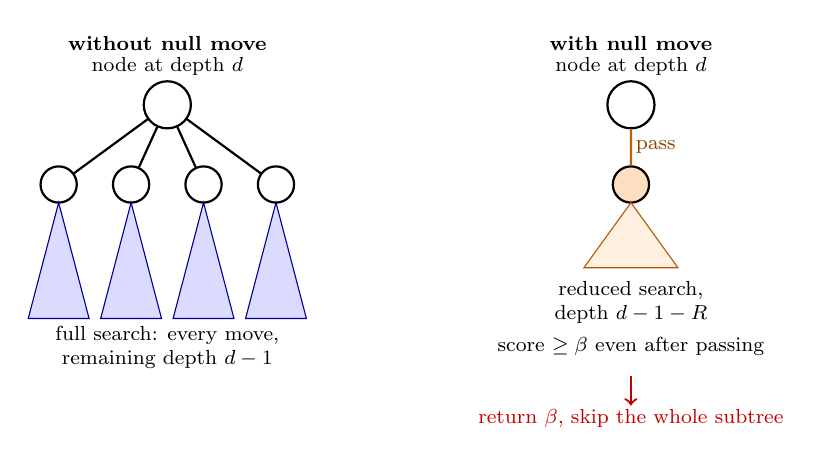
\begin{tikzpicture}[
  scale=0.92, transform shape, font=\small,
  nd/.style={draw, thick, circle, minimum size=6.5mm, inner sep=0pt},
  lbl/.style={font=\footnotesize, inner sep=1.5pt}
]
% ---------------- left: what the node would cost --------------------------
\begin{scope}
  \node[nd] (r) at (2,2.6) {};
  \node[lbl, anchor=south] at (2,2.95) {node at depth $d$};
  \foreach \i/\x in {1/0.5,2/1.5,3/2.5,4/3.5}{
    \node[nd, minimum size=5mm] (m\i) at (\x,1.5) {};
    \draw[thick] (r) -- (m\i);
  }
  \foreach \i/\x in {1/0.5,2/1.5,3/2.5,4/3.5}
    \draw[fill=blue!14, draw=blue!55!black] (\x,1.25) -- (\x-0.42,-0.35) -- (\x+0.42,-0.35) -- cycle;
  \node[lbl, align=center] at (2,-0.75) {full search: every move,\\remaining depth $d-1$};
  \node[font=\footnotesize\bfseries] at (2,3.45) {without null move};
\end{scope}
% ---------------- right: the null-move probe ------------------------------
\begin{scope}[xshift=6.4cm]
  \node[nd] (R) at (2,2.6) {};
  \node[lbl, anchor=south] at (2,2.95) {node at depth $d$};
  \node[nd, minimum size=5mm, fill=orange!25] (P) at (2,1.5) {};
  \draw[thick, orange!75!black] (R) -- node[lbl, right, text=orange!55!black] {pass} (P);
  \draw[fill=orange!12, draw=orange!70!black] (2,1.25) -- (1.35,0.35) -- (2.65,0.35) -- cycle;
  \node[lbl, align=center, anchor=north] at (2,0.22) {reduced search,\\depth $d-1-R$};
  \node[lbl, align=center, anchor=north] at (2,-0.55)
    {score $\geq \beta$ even after passing};
  \draw[->, red!75!black, thick] (2,-1.15) -- (2,-1.55);
  \node[lbl, align=center, anchor=north, text=red!75!black] at (2,-1.55)
    {return $\beta$, skip the whole subtree};
  \node[font=\footnotesize\bfseries] at (2,3.45) {with null move};
\end{scope}
\end{tikzpicture}
\caption{Null-move pruning. Instead of searching every move at full depth (left),
the engine first lets the side to move pass and searches the resulting position
to a reduced depth (right). If the position is still good enough to exceed
$\beta$ despite this handicap, the node is assumed to be beyond the opponent's
reach and the subtree is skipped. The saving is large because the probe is both
shallower and single-branched, but the inference is heuristic: it fails in
zugzwang, where passing would be an improvement rather than a concession.}
\label{fig:nullmove}
\end{figure}

The pruning is performed inside \texttt{negamax}, after the transposition table
probe but before the moves are generated and ordered. The engine plays a null
move via \texttt{board.make\_null\_move()}, searches the resulting position to a
reduced depth $d-1-R$ with a null window around $\beta$ (realized as
$[-\beta, -\beta+1]$ in the Negamax formulation), and restores the position with
\texttt{board.pop\_null\_move()}. If the returned score satisfies
$-\text{score} \ge \beta$, the node fails high and $\beta$ is returned directly.
The number of such cutoffs is tracked in the \texttt{null\_cutoffs} counter for
the experimental instrumentation.

Because null-move pruning is a heuristic rather than an exact technique, it is
guarded by several conditions. The reduced search is only attempted when all of
the following hold:
\begin{itemize}
    \item pruning is enabled and this node was not already reached through a null
    move (\texttt{can\_null}); two consecutive passes are never searched, as they
    correspond to no meaningful line of play,
    \item the node is not the root ($ply > 0$), since the root must always return
    a real best move,
    \item the remaining depth is at least \texttt{min\_depth}; below this the
    reduced search would be too shallow to justify the risk,
    \item $\beta$ is not already a mate score
    ($|\beta| < \texttt{kMate} - \texttt{kMateWindow}$), because a fabricated
    move would distort mate distances,
    \item the side to move is not in check, since passing while in check would
    leave the king en prise,
    \item the side to move still has non-pawn material
    (\texttt{has\_non\_pawn\_material}); in pawn-only endgames zugzwang makes
    passing frequently favourable, which would invalidate the pruning assumption.
\end{itemize}

As in the rest of the search, an aborted reduced search is not trusted: if the
null-move search is terminated by a hard stop, the abort is propagated upward and
no cutoff is derived from the incomplete result. The behaviour is controlled by a
\texttt{NullMoveConfig} structure exposing whether the technique is enabled, the
minimum remaining depth (\texttt{min\_depth}, default $3$), and the depth
reduction (\texttt{reduction}, default $2$). All three are exposed as the UCI
options \texttt{NullMove}, \texttt{NullMoveMinDepth}, and
\texttt{NullMoveReduction}, so the pruning can be toggled and tuned without
recompiling.

\subsubsection{Transposition Table Integration}

The motivation for the table is that the game tree is not, strictly speaking, a
tree. Different sequences of moves frequently lead to the identical position, so
the same node appears many times over at the same depth. A plain recursive search
has no way of noticing this and re-solves each occurrence from scratch, which is
pure duplicated work. \cref{fig:transposition} shows the effect in its smallest
form. Storing results under a hash of the position turns the traversal from a
tree into a directed acyclic graph and lets the second occurrence be answered
from memory. Since the number of such collisions grows with depth, this is one of
the few techniques whose benefit increases rather than decreases as the search
gets deeper, which is also why the same table can be carried across moves
(\cref{subsec:tree_reuse}).

\begin{figure}[ht]
\centering
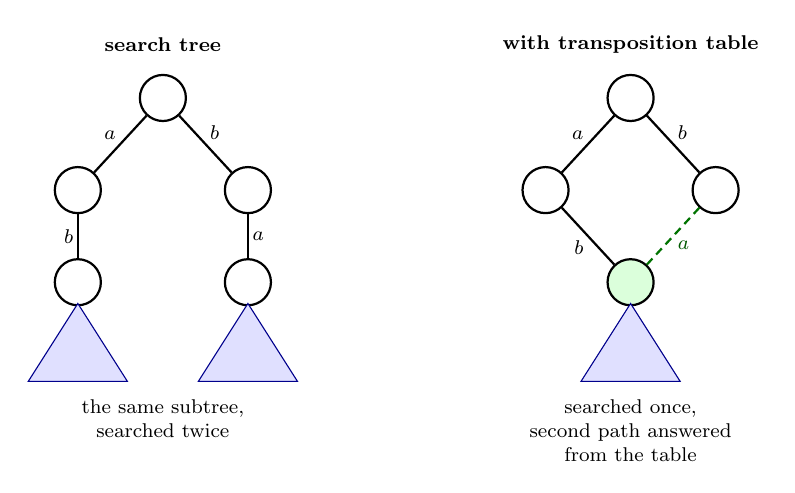
\begin{tikzpicture}[
  scale=0.9, transform shape, font=\small,
  nd/.style={draw, thick, circle, minimum size=6.5mm, inner sep=0pt},
  lbl/.style={font=\footnotesize, inner sep=1.5pt}
]
% ---------------- left: plain tree ----------------
\begin{scope}
  \node[nd] (r) at (2,3) {};
  \node[nd] (x1) at (0.8,1.7) {};
  \node[nd] (x2) at (3.2,1.7) {};
  \node[nd] (y1) at (0.8,0.4) {};
  \node[nd] (y2) at (3.2,0.4) {};
  \draw[thick] (r) -- node[lbl,above left] {$a$} (x1);
  \draw[thick] (r) -- node[lbl,above right] {$b$} (x2);
  \draw[thick] (x1) -- node[lbl,left] {$b$} (y1);
  \draw[thick] (x2) -- node[lbl,right] {$a$} (y2);
  \draw[fill=blue!12, draw=blue!55!black] (0.8,0.1) -- (0.1,-1.0) -- (1.5,-1.0) -- cycle;
  \draw[fill=blue!12, draw=blue!55!black] (3.2,0.1) -- (2.5,-1.0) -- (3.9,-1.0) -- cycle;
  \node[lbl, align=center, anchor=north] at (2,-1.20) {the same subtree,\\searched twice};
  \node[font=\footnotesize\bfseries] at (2,3.75) {search tree};
\end{scope}
% ---------------- right: DAG ----------------
\begin{scope}[xshift=6.6cm]
  \node[nd] (R) at (2,3) {};
  \node[nd] (X1) at (0.8,1.7) {};
  \node[nd] (X2) at (3.2,1.7) {};
  \node[nd, fill=green!14] (Y) at (2,0.4) {};
  \draw[thick] (R) -- node[lbl,above left] {$a$} (X1);
  \draw[thick] (R) -- node[lbl,above right] {$b$} (X2);
  \draw[thick] (X1) -- node[lbl,below left] {$b$} (Y);
  \draw[thick, densely dashed, green!45!black] (X2) --
        node[lbl,below right, text=green!35!black] {$a$} (Y);
  \draw[fill=blue!12, draw=blue!55!black] (2,0.1) -- (1.3,-1.0) -- (2.7,-1.0) -- cycle;
  \node[lbl, align=center, anchor=north] at (2,-1.20) {searched once,\\second path answered\\from the table};
  \node[font=\footnotesize\bfseries] at (2,3.75) {with transposition table};
\end{scope}
\end{tikzpicture}
\caption{Transpositions. Playing move $a$ and then $b$ leads to exactly the same
position as playing $b$ and then $a$, so a plain recursive search explores the
identical subtree twice (left). A transposition table stores the result of the
first visit under a hash of the position, so the second path finds it already
solved and returns immediately (right). Real search trees contain vastly more
such convergences than this minimal example suggests.}
\label{fig:transposition}
\end{figure}

The search consults the transposition table early in \texttt{negamax} via
\texttt{tt.probe(key, depth, alpha, beta, ply, ...)}. A successful probe may:
\begin{itemize}
    \item return an \texttt{EXACT} score,
    \item produce a safe cutoff using stored \texttt{LOWER\_BOUND} or
    \texttt{UPPER\_BOUND} information.
\end{itemize}

In addition, the table provides a stored best move (\texttt{tt\_move}) which is
used for move ordering. Since transposition table entries may be stale or collide,
the implementation verifies the move's legality before using it; illegal TT moves
are discarded.

After searching a node, the result is stored via \texttt{tt.store(...)} together
with the depth, bound type, and the best move found at that node. Mate scores are
encoded in a TT-safe form using the ply (via \texttt{to\_tt\_score} /
\texttt{from\_tt\_score}) so that mate distances remain consistent across
different search depths.

\subsubsection{Search Tree Reuse Across Searches}
\label{subsec:tree_reuse}

The transposition table is not only used within a single search invocation but
also serves as the engine's mechanism for resuming previous search trees. The
table is a member of the engine instance and is deliberately \emph{not} cleared
between searches. When a new search starts, \texttt{reset\_search\_state()}
only calls \texttt{tt.new\_search()}, which advances an internal generation
counter; all stored entries remain accessible. A full \texttt{tt.clear()} is
performed only when the UCI command \texttt{ucinewgame} signals that an
entirely new game begins.

This design directly implements the idea of continuing an earlier computation.
After the engine has played a move and the opponent has answered, the new root
position lies inside the tree that was explored during the previous search.
Probing the persistent table therefore immediately recovers large parts of the
earlier work:
\begin{itemize}
    \item \textbf{Score reuse:} entries stored with sufficient depth yield
    exact scores or safe bound cutoffs without re-searching the corresponding
    subtrees.
    \item \textbf{Move ordering reuse:} stored best moves from the previous
    search guide the move ordering of the new search from the very first
    iteration, which is exactly the situation in which Principal Variation
    Search and Alpha-Beta pruning are most effective.
\end{itemize}

The generation counter implements a soft aging scheme rather than hard
invalidation. The replacement policy prefers overwriting entries from older
generations and entries with lower depth, so stale information gradually
disappears as the game progresses while still being available as long as it is
not displaced. In combination with iterative deepening, this means consecutive
searches behave less like independent computations and more like one continuous
search that is deepened and re-rooted as the game advances.

Keeping the table alive across searches has one consequence that a table cleared
per search does not have: a stored move outlives the position it was generated
for. Since the table is indexed by a truncated key, two different positions can
map to the same entry, and the move handed back then describes pieces that are no
longer where it expects them. Such a move is not merely bad, it is not playable at
all, and applying it would corrupt the board rather than just cost search time.
Every move taken from the table is therefore validated against the current
position before it is used as an answer: it has to be one the move generator
produces here, and it must not leave the own king in check. Moves that come
straight from the generator need no such check, they are pseudo-legal by
construction, so the validation is confined to the few places where a move of
foreign origin enters the search.

\subsubsection{Move Ordering and Heuristics}
\label{subsec:move_ordering}

Move ordering is implemented in \texttt{search::heuristics::order\_moves}.
The ordering score combines several standard heuristics, all of which are
surveyed by Marsland~\cite{marsland1986review}:
\begin{itemize}
    \item \textbf{TT/PV move first:} if a transposition table move exists, it
    receives a large bonus and is sorted to the front.
    \item \textbf{Captures before quiet moves:} captures are prioritized using a
    MVV-LVA-inspired score (most valuable victim / least valuable attacker),
    with a special case for en-passant.
    \item \textbf{Killer moves:} for each ply, the engine tracks up to two quiet
    moves that previously caused beta cutoffs and boosts them in ordering.
    \item \textbf{History heuristic}~\cite{schaeffer1989history}\textbf{:} a 3D
    table indexed by side, from-square, and to-square accumulates bonuses (scaled
    by depth squared) for quiet moves that caused cutoffs, and the accumulated
    score is added during ordering.
\end{itemize}

Killer and history updates are performed only on beta cutoffs and only for quiet
moves. This avoids polluting these tables with captures and ensures that the
heuristics reflect moves that are generally useful for pruning rather than
tactical one-offs.

\subsubsection{Debugging and Instrumentation}

The search provides UCI-compliant reporting via \texttt{print\_info}, including
depth, selective depth, time, nodes, NPS, and either centipawn score or mate
distance (converted from the internal mate representation). Additionally, a
configurable debug facility can emit search health statistics, transposition
table statistics, root move ordering, and principal variation output. This
instrumentation supports the experimental goal of this thesis by making search
behavior observable and reproducible.

\section{Time Management and Constraints}
\label{sec:time_management}

In practical chess engines, search is not only limited by depth but often by a
set of external constraints such as time, node budgets, or explicit stop
signals. In this engine, all stopping conditions for a single search invocation
are bundled in an immutable constraint object, which is initialized once before
the search starts and treated as read-only during the search.

A key design goal is that the search code itself does not depend on UCI parsing
details. Instead, the UCI layer produces a fully specified \texttt{SearchConstraints}
instance, and the search only consults this object (and a stop flag) to decide
when to terminate.

\subsection{Unified Constraint Model}

The engine uses a dedicated \texttt{SearchConstraints} structure to describe how
a search is controlled and when it should terminate. This structure unifies all
search modes under a single interface and avoids scattered termination logic
across the search code.

A constraint instance contains:
\begin{itemize}
    \item a \textbf{search mode} determining which criteria are active,
    \item an optional \textbf{fixed move time} (\texttt{movetime\_ms\_}),
    \item an optional \textbf{fixed depth} (\texttt{depth\_}),
    \item an optional \textbf{node limit} (\texttt{nodes\_}),
    \item and a \textbf{time budget} object (\texttt{budget\_}) used for time-managed searches.
\end{itemize}

To simplify checks in the search, convenience predicates such as
\texttt{has\_fixed\_depth()}, \texttt{has\_node\_limit()}, and \texttt{has\_movetime()}
are provided.

\subsection{Search Modes}

The active search behavior is selected via \texttt{SearchType}. The engine
supports the following modes:
\begin{itemize}
    \item \textbf{Normal:} Tournament-style time management with iterative
    deepening (default UCI behavior). Time allocation is derived from the clock
    settings and stored in \texttt{budget\_}.
    \item \textbf{FixedTime:} Search for a fixed amount of time specified by
    \texttt{movetime\_ms\_} (UCI \texttt{go movetime}).
    \item \textbf{FixedDepth:} Search to a fixed depth only, determined by
    \texttt{depth\_}, without relying on time control.
    \item \textbf{NodeLimit:} Search until a fixed number of nodes specified by
    \texttt{nodes\_} has been explored.
    \item \textbf{Infinite:} Search indefinitely until an external stop command
    is received (UCI \texttt{go infinite}).
    \item \textbf{Ponder:} Search during the opponent’s time. The engine
    continues searching until it is either stopped or the predicted opponent
    move is played, at which point the search can be continued or restarted.
\end{itemize}

This mode-based design enables a clean separation between the UCI interface
(which interprets the \texttt{go} command) and the search itself (which only
consults the active constraints).

\subsection{Time Budgets: Structure and Arming}

Time-based searches (Normal / FixedTime) rely on \texttt{TimeControl} stored in
\texttt{SearchConstraints::budget\_}. The budget distinguishes a \emph{soft} and a
\emph{hard} limit:
\begin{itemize}
    \item \textbf{Soft deadline:} preferred stopping point, checked only at safe
    boundaries (between completed iterations of iterative deepening).
    \item \textbf{Hard deadline:} strict upper bound that must not be exceeded,
    checked frequently throughout the search (including quiescence).
\end{itemize}

\paragraph{Unarmed Budgets for Non-time Modes}
A crucial implementation detail is that \texttt{budget\_} is explicitly
\emph{disarmed} for non-time-based modes. Concretely, deadlines are set to zero,
so \texttt{soft\_time\_up(...)} and \texttt{hard\_time\_up(...)} always return
false. This ensures that depth-limited and node-limited search do not depend on
any timing state.

\paragraph{Arming the Budget Before Search}
Immediately before a time-managed search begins, \texttt{TimeManager::init\_search}
is called. This function captures the current monotonic time
(\texttt{now\_ms()}) as the start timestamp and derives absolute deadlines:
\[
\texttt{soft\_deadline\_ms\_} = \texttt{start\_ms\_} + \texttt{soft\_ms\_}, \qquad
\texttt{hard\_deadline\_ms\_} = \texttt{start\_ms\_} + \texttt{hard\_ms\_}.
\]
From this point onward, the budget object is treated as read-only.

\subsection{Termination Conditions in the Search}

The engine enforces termination using a combination of (i) an external stop flag,
(ii) the hard deadline, and (iii) an optional node limit. These checks are
centralized in \texttt{ChessBot::hard\_stop()}, which is called frequently inside
the main search and quiescence.

\paragraph{Hard Stop Checks}
The stop check follows the order shown in \cref{algo:hardstop}: first an external
flag, then the hard time deadline, then the node limit. If any condition is met,
the search aborts immediately and returns a special ``aborted'' result to the
caller.

\begin{algorithm}[ht]
\DontPrintSemicolon
\KwIn{Current time $now$}
\KwOut{\texttt{true} iff the search must terminate immediately}

\If{\texttt{stop\_requested} is set}{
    \Return \texttt{true}\;
}
\If{\texttt{budget\_.hard\_time\_up(now)}}{
    \Return \texttt{true}\;
}
\If{\texttt{has\_node\_limit()} \textbf{and} \texttt{nodes >= nodes\_}}{
    \Return \texttt{true}\;
}
\Return \texttt{false}\;
\caption{Immediate termination check (\texttt{hard\_stop()}).}
\label{algo:hardstop}
\end{algorithm}

\paragraph{Soft Stop in Iterative Deepening}
In contrast to the hard deadline, the \emph{soft} deadline is checked only after
a complete iteration has finished. This ensures that the engine does not stop
mid-iteration, which would otherwise risk returning an unstable or partially
explored root result. The structure is summarized in \cref{algo:softstop}.

\begin{algorithm}[ht]
\DontPrintSemicolon
\KwIn{Board position $P$}
\KwOut{Best move found within the budget}

$bestMove \gets$ legal fallback move\;
\For{$d \gets 1,2,3,\dots$}{
    $(score, aborted) \gets$ depth-limited root search at depth $d$\;
    \If{$aborted$}{
        \textbf{break}\tcp*{do not trust partial iteration}
    }
    $bestMove \gets$ move from completed iteration\;
    \If{\texttt{budget\_.soft\_time\_up(now)}}{
        \textbf{break}\tcp*{stop cleanly after a full iteration}
    }
}
\Return $bestMove$\;
\caption{Soft stopping policy at iteration boundaries (iterative deepening).}
\label{algo:softstop}
\end{algorithm}

\subsection{Summary}

The engine models time control and other stopping criteria using a single,
immutable \texttt{SearchConstraints} object. By activating different termination
rules depending on \texttt{SearchType} and by explicitly arming or disarming time
budgets, the implementation remains robust and easy to analyze.

Most importantly, the implementation distinguishes between \emph{hard} stopping
conditions, which are enforced immediately inside the recursive search, and a
\emph{soft} stopping condition, which terminates the search cleanly between
iterations of iterative deepening. This separation is essential for making
time-constrained iterative deepening comparable to fixed-depth search in later
experiments, since it ensures that the engine always returns the best move from
the last fully completed depth.

\subsection{Evaluation Function}
\label{sec:evaluation_function}

This section describes the static evaluation function used by the engine. Since
the search explores only a limited portion of the game tree, a heuristic
evaluation is required to estimate the quality of non-terminal positions. The
implemented evaluation follows a classical \emph{tapered} approach with separate
midgame (MG) and endgame (EG) scores, piece-square tables (PSQT), a phase-based
interpolation scheme, and a tempo bonus.

\subsubsection{Material Model}
\label{subsec:material_model}

The evaluation assigns a material value to each piece type. Material is counted
for both sides and is added to the positional contribution of the corresponding
piece-square table. Conceptually, for a piece on square $s$, the score is:
\[
\text{score}(p,s) = \text{material}(p) + \text{psqt}(p,s).
\]
In the implementation, material values are used in two variants: a midgame value
and an endgame value. This is consistent with the idea that the relative
importance of pieces changes over the course of a game (e.g., kings become more
active in endgames).

\subsubsection{Piece-Square Tables (PSQT)}
\label{subsec:psqt}

Positional preferences are encoded using piece-square tables. For each piece
type, the engine stores a 64-entry table for midgame and endgame, assigning a
positional bonus (or penalty) to each square. This model captures common chess
principles such as centralization, piece activity, and king safety without
explicit feature engineering.

The implementation uses a single table orientation and mirrors squares for the
white pieces by applying a rank flip. Concretely, for a board index $i$,
white pieces use index $i \oplus 56$, while black pieces use $i$ directly. This
ensures that both colours share the same PSQT semantics relative to their
respective perspective.

\subsubsection{Midgame and Endgame Separation}
\label{subsec:mg_eg}

Instead of a single score, the evaluation computes two scores:
\begin{itemize}
    \item $MG$: midgame score (material + PSQT using MG tables),
    \item $EG$: endgame score (material + PSQT using EG tables).
\end{itemize}

The engine accumulates these values separately for both sides. The final score
is then expressed from the perspective of the \emph{side to move}. This is
implemented by subtracting the opponent's accumulated values from the values of
the player whose turn it is.

\subsubsection{Game Phase Interpolation}
\label{subsec:phase_interpolation}

To smoothly transition between midgame and endgame behavior, the engine uses a
tapered evaluation. A game-phase value is computed as the sum of per-piece phase
contributions. The resulting phase is clamped to a maximum of $24$, yielding:
\[
mgPhase = \min(24, \text{phase}(P)), \qquad egPhase = 24 - mgPhase.
\]
The final evaluation is obtained by linear interpolation:
\[
Eval(P) = \frac{MG(P)\cdot mgPhase + EG(P)\cdot egPhase}{24}.
\]
This approach is commonly used in classical engines, as it avoids abrupt
evaluation changes and provides a simple, interpretable blending scheme.

\begin{figure}[ht]
\centering
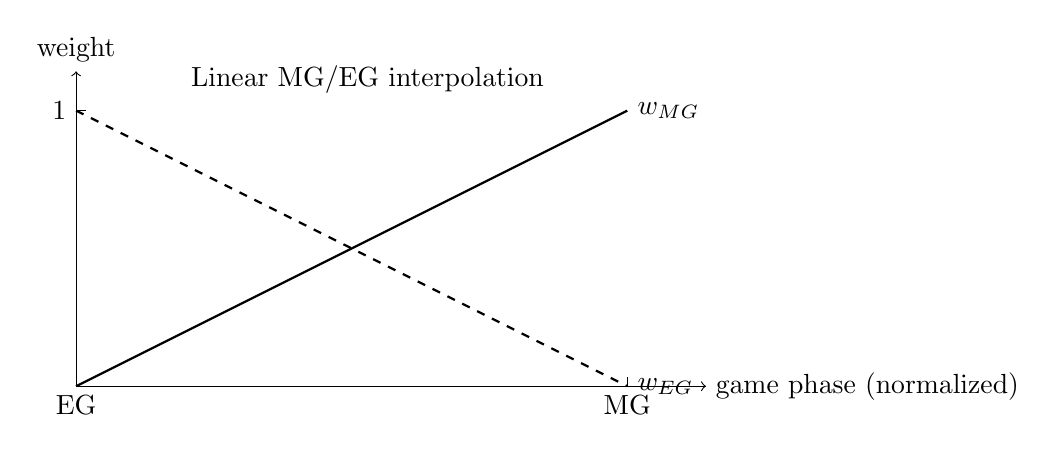
\begin{tikzpicture}[scale=1.0]
  \draw[->] (0,0) -- (8,0) node[right] {game phase (normalized)};
  \draw[->] (0,0) -- (0,4) node[above] {weight};

  % mg weight line: 0..1
  \draw[thick] (0,0) -- (7,3.5) node[right] {$w_{MG}$};
  % eg weight line: 1..0
  \draw[thick,dashed] (0,3.5) -- (7,0) node[right] {$w_{EG}$};

  % ticks
  \foreach \x/\lab in {0/EG,7/MG}{
    \draw (\x,0) -- (\x,0.12);
    \node[below] at (\x,0) {\lab};
  }
  \draw (0,3.5) -- (0.12,3.5);
  \node[left] at (0,3.5) {1};

  \node at (3.7,3.9) {Linear MG/EG interpolation};
\end{tikzpicture}
\caption{Tapered evaluation: midgame and endgame weights vary linearly with the
game phase.}
\label{fig:tapered_eval}
\end{figure}

\subsubsection{Tempo Bonus}
\label{subsec:tempo_bonus}

A constant tempo bonus is added to the final score to reflect the advantage of
having the next move. In the implementation, the returned evaluation is:
\[
Eval_\text{final}(P) = Eval(P) + 20.
\]
Since the engine evaluates positions from the perspective of the side to move,
this constant shifts the score slightly in favor of the player whose turn it is,
encouraging initiative and reducing symmetry artifacts.

\subsubsection{Algorithmic Summary}
\label{subsec:eval_algorithm}

\begin{algorithm}[ht]
\DontPrintSemicolon
\KwIn{Board position $P$}
\KwOut{Static evaluation score from the perspective of the side to move}

Initialize $mg[2]\gets 0$, $eg[2]\gets 0$, $phase\gets 0$\;

\For{$i \gets 0$ \KwTo $63$}{
    $piece \gets P[i]$\;
    $phase \gets phase + phaseValue(piece)$\;
    \uIf{$piece$ is white}{
        $idx \gets i \oplus 56$\tcp*{mirror for white}
        $mg[W] \gets mg[W] + MG\_PSQT(piece, idx) + MG\_MAT(piece)$\;
        $eg[W] \gets eg[W] + EG\_PSQT(piece, idx) + EG\_MAT(piece)$\;
    }
    \uElseIf{$piece$ is black}{
        $idx \gets i$\;
        $mg[B] \gets mg[B] + MG\_PSQT(piece, idx) + MG\_MAT(piece)$\;
        $eg[B] \gets eg[B] + EG\_PSQT(piece, idx) + EG\_MAT(piece)$\;
    }
}

$mgPhase \gets \min(24, phase)$\;
$egPhase \gets 24 - mgPhase$\;

Compute $MG(P)$ and $EG(P)$ as difference between side-to-move and opponent\;
$Eval(P) \gets \big(MG(P)\cdot mgPhase + EG(P)\cdot egPhase\big) / 24$\;

\Return $Eval(P) + 20$\tcp*{tempo}
\caption{Static evaluation with MG/EG separation, tapered interpolation, and tempo bonus.}
\label{algo:evaluation}
\end{algorithm}

\subsubsection{Limitations of the Evaluation}
\label{subsec:eval_limitations}

The evaluation is intentionally simple and focuses on material and PSQT-based
positional features. This makes it fast and easy to analyze, but it also implies
several limitations:
\begin{itemize}
    \item \textbf{Limited feature set:} Pawn structure (isolated/doubled/passed
    pawns), mobility, rook activity on open files, bishop pair, and advanced king
    safety concepts are not modeled explicitly.
    \item \textbf{No explicit drawishness detection:} The evaluation does not
    implement specialized scaling for fortress-like positions, opposite-coloured
    bishop endgames, or other draw-prone material configurations.
    \item \textbf{Constant tempo term:} The tempo bonus is a fixed constant and
    does not depend on phase or position characteristics.
    \item \textbf{No incremental evaluation:} The score is computed by scanning
    all 64 squares, rather than updating evaluation terms incrementally during
    make/unmake.
\end{itemize}

Despite these limitations, the evaluation is sufficient for the primary focus of
this thesis, namely the investigation of search behavior and iterative deepening
under time constraints. A stronger evaluation can be integrated later without
changing the surrounding search architecture.
